\subsection{GIMME-2}
The GIMME-2 board system is equipped with two 10 Megapixel image sensors. The GIMME-2 has a zynq processor which has an ARM Cortex A9 dual-core processor and FPGA in the same chip. The board has 8 GB of RAM . There is a slot for external memory storage. The operating system installed on the GIMME-2 board is Peta Linux.  All instructions for  building the operating system on GIMME-2 can be found in appendix \ref{GIMME2}.
	
The system retrieves missions from the decision center and sends back information according to the given mission. Fig. \ref{Gimme_f} explains how the system works. 
\begin{center}
\begin{figure}
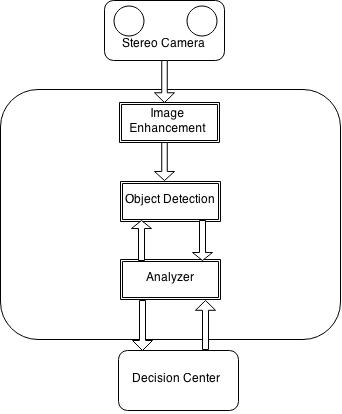
\includegraphics[height=10cm]{./Images/GIMME-2/f}
\captionsetup{singlelinecheck=off}
\caption[hej]{\label{Gimme_f}
\begin{itemize}
\item Stereo Cameras: continuously takes images underwater.
\item Image Enhancement: Enhance incoming images from stereo camera.
\item Analyzer: Analyze incoming mission(type of object to detect) and send back required parameters to Mission control center.
\item Object Detection: Detect objects according to the Analyzer and send back feedback to the Analyzer.
\end{itemize}}

\end{figure}
\end{center}

\subsubsection{Operating system}
The operating system used on the GIMME-2 board is Peta Linux 2014.3 customized by Xilinx for Zynq processor which is based on the vanilla kernels. There are two ways the user can interact with the GIMME-2 board either through a serial port interface (USB cable ) or through SSH client(Ethernet cable).
Creating  a bootable Linux for zynq on GIMME-2 board  is challenging due to the fact that the files available on the Xilinx website are mostly for the Zynq evaluation board. The files that are necessary for booting Linux have to be built from scratch, the procedure and tools used for building these files are described in details in Xilinx wiki web site \cite{xilinxuserguide}. 
At first the First Stage Boot Loader (FSBL) starts and does the early system initialization then the universal bootloader starts which loads the kernel image and the wrapped ramdisk image.

\subsubsection{Vision system software}
The software in the vision system is a major issue especially since it is dealing with live captured images in underwater conditions, which have changing lighting conditions that will affect the image detection system.

A vision system has been made using OpenCV to deal with all the issues that the vision system can face. 

In order to have a better calibration between the GIMME-2 cameras and the real live values a red light detection system has been made which was the start for building  the vision system.

\subsubsection{OpenCV for GIMME-2}
OpenCV has been used in order to implement vision methods  since it has a lot of functions that could be used to have a better detection and  enhance the underwater image, the challenge was to build the OpenCV for GIMME-2 board. Arm-linux-gnueabi cross compiler has been used for building OpenCV for GIMME-2. All instructions of building OpenCV for GIMME-2 can be found in appendix \ref{OPENCV}.

\subsubsection{Image Enhancement} 
Underwater images are not clear, when the depth increases, the amount of light on objects decreases and the light distribution becomes irregular \cite{Image_Enhancement}. So before further image processing, enhancement of  incoming images from cameras has been done  by  converting the image to YUV( Y referred to as luminance or luma, while U and V is the chroma) color space and perform Contrast Limited Adaptive Histogram Equalization (CLAHE) on the Luminescence (Y) channel for improving image contrast \cite{Image_Enhancement}. Dilate and erode which are functions used in OpenCV are also used to enhance input images.

\subsubsection{Red Light Detection}
Detecting the red light is very important since that it is the base that all the detection in the vision system depends on especially for the real life calibration. Working with OpenCV, two red light detection systems has been made. The first depends on the red light channels inside the image which called the red boost method \cite{Red_boost_Method}. The second depends on taking the histogram of the red channel inside the picture and back project the most red part in the histogram which is called the histogram method \cite{Histogram_Method}.

The red boost method starts with reading the BGR image and split it into three channels red, green and blue. Then take away the green and blue and  keep the red only. 
Once the green and blue colours is taken away use the multiply function used in OpenCV to boost up the red color only and save the final image in a matrix of type Mat. 
After that, threshold the red boosted using threshold image function used in OpenCV and keep only the highest red and save the threstholded image. The threstholded image will be sent to the moment class used in OpenCV to get the x and y of the center of the detected red.
 
Histogram method works by finding the histogram of the image and then back project the highest red position in the source image. It starts with reading the BGR image and then split it into three planes. Using the split function in OpenCV a green, blue and red plane will be generated and sent into the calcHist function used in OpenCV with a specific histogram range depends on the hue range for the red colour. 

Once the histogram calculation is done for the three planes a normalization is required to assure that the histogram is in the range for the BGR image. Once that is done the highest red can be detected by calling the calcBackProject function in OpenCV \cite{Histogram_Method_in_opencv} which will threshold the image using the hue range  and by that will detect the red light, and this image will be sent to the moment class to get the x and y of the center of the detected red. 

\subsubsection{Object Detection}
For object detection, template matching and shape matching has been tested, but they are not good when the object is rotated or scaled; the irregular light distribution underwater would mean having extensive number of  templates which would be time consuming so feature detection algorithms and classification algorithms has been used to detect the required objects and additional complex objects.

Once the object is detected by the stereo camera, the system will find the necessary parameters. It sends back the x coordinates of the object in both images and then the distance is determined by the difference between these two coordinates.

The distance is found by multiplying F (the focal length of the camera) with B (the distance between the cameras) and divide the answer by disparity (the difference between the x coordinates from left and right images) as seen in equation \ref{equation:1}, and then the final answer is multiplied with a calibrated value to get the distance in real life\cite{Stereo_Camera} \cite{Find_distance}.
\begin{equation}\label{equation:1}
Distance = (F*B)/disparity
\end{equation} 
To find the yaw of the detected object the y coordinates of the detected object is needed and the distance to the object and some gain value found from a lots of testing in real life conditions.
First multiply the difference in x between the object and the center with the distance to the object and the gain value as seen in equation \ref{equation:2}, and then divide the answer by 100 to get the final value in meters as seen in equation \ref{equation:3}.
\begin{equation}\label{equation:2}
pos y= pos y (x difference) * Gain * distance
\end{equation} 
\begin{equation}\label{equation:3}
pos y=pos y/100
\end{equation} 
Finally to find the yaw value of the object the mathematical function arctan is needed with parameters for (pos y) and distance as seen in equation \ref{equation:4}.
\begin{equation}\label{equation:4}
Yaw=atan2 (pos y , distance)*(180/PI)
\end{equation} 
Finding the z position of the detected object  can be done mathematically with the need of distance to the object and some gain value found from a lot of testing in real life condition and finally the y difference between the object and the center as seen in equation \ref{equation:5} and \ref{equation:6} .
\begin{equation}\label{equation:5}
pos z =  pos z  (y difference) *Gain*distance
\end{equation} 
\begin{equation}\label{equation:6}
pos z =  pos z /100.
\end{equation} 

\subsubsection{SURF Algorithm}
 SURF(speeded up robust features)  is a fast, and more accurate algorithm compared to others \cite{SURF_Speed}. When using SURF four steps should be followed:
 \begin{enumerate}
\item Key points selection from both images (object and scene). 
\item Eextraction of descriptors from those key points.
\item Match descriptors by matcher.
\item Analyze  matches \cite{SURF}.
 \end{enumerate}

For matching flann matcher and knn (k-nearest neighbor) matcher has been used, and knn give. Better results. As a final result of SURF it can be a very useful method for complex objects and it can detect some of required objects, but not all of them because they do not have too many features and edges.

The SURF algorithm APIs is not included within the OpenCV repository is intended for development of so called extra modules. All instructions of building extra modules with OpenCV for GIMME-2 can be found in \ref{OPENCV}.

\subsubsection{Classification}
One of the best object detection methods is the Haar Cascade Classifiers. It is a machine learning based method, which uses a cascade trained by hundreds of sample pictures called positive and negative images \cite{Haar_Classification}.

The haar training is the most difficult and time consuming part of the haar cascade method. Once the negative and  positive images is gathered the user can start  making the sample images which combine the negative and the positive images in one file once the samples images is finished the final step left is to start the training and generate the Haar trained file.

The instructions for training your own Haar Cascade can be found in \cite{Haar_Cascade_Training} and
 \cite{Opencv_Haar_Training}.
 
\subsubsection{Gate Detection}
For gate detection the enhanced image has been converted to HSV (Hue, Saturation and Value) and segmented for a specific color. Edge detection is used to separate desired edges, which makes it possible to find contours.